\section{Descripción de los datos del estudio}
\label{sec:datos}
\citet{jimenez-tejaFirstJointMUSE2024} estudiaron la luz intracumular (ICL) de \cluster{} (de ahora en adelante, \clust{}) en varias longitudes de onda del espectro visible y el infrarrojo cercano, para lo que emplearon datos recogidos por el Telescopio Espacial Hubble (HST), el Telescopio Espacial James Webb (JWST), y el espectrógrafo Multi Unit Spectroscopic Explorer (MUSE) del Very Large Telescope (VLT) perteneciente al European Southern Observatory (ESO). En este trabajo partiremos de los mismos datos para estudiar las shells de la BCG. \par

\clust{} está situado a un redshift \(z=0,234\), \(21^{\text{h}}29^{\text{m}}40^{\text{s}}\) de ascensión recta y \(+00^{\circ} 05^{\prime}18^{\prime\prime}.8\) de declinación. Suponiendo un modelo cosmológico estándar con \(H_0 = 70 \: \text{km} \: \text{s}^{-1} \: \text{Mpc}^{-1}\), \(\Omega_m = 0,3\) y \(\Omega_\Lambda = 0,7\); dicho \(z\) se corresponde con un instante \(\sim 10,7\) Gyr después del Big Bang y con una escala espacial de \(3,722\) kpc/arcsec \citep{wrightCosmologyCalculatorWorld2006}.\par

Si bien este no es el primer estudio fotométrico de las shells de una galaxia, sí es la primera vez que se analizan las de un objeto tan lejano utilizando los datos de estos tres telescopios al mismo tiempo (p. ej. \citet{mihosStelLARPOPULATIONSOUTER2013} estudiaron una galaxia situada a \(z = 0,003\)\footnote{\url{http://ned.ipac.caltech.edu/cgi-bin/objsearch?objname=Messier+49&extend=no&hconst=73&omegam=0.27&omegav=0.73&corr_z=1&out_csys=Equatorial&out_equinox=J2000.0&obj_sort=RA+or+Longitude&of=pre_text&zv_breaker=30000.0&list_limit=5&img_stamp=YES}} con un telescopio terrestre de la CWRU de Ohio). Como veremos, la resolución superior de JWST y sus mayores capacidades para la observación en el infrarrojo suponen un salto cualitativo para la caracterización de objetos de bajo brillo superficial como las shells. \par

Todos los telescopios publican sus observaciones según el estándar del formato \textit{.fits}, que incluye en un mismo archivo dos tipos de datos. \textit{Data} es el vector de la imagen (en el caso de la espectroscopía, el cubo de datos) a estudiar, en nuestro caso ya calibrada, procesada y combinada en un mosaico mediante la \textit{pipeline} correspondiente a cada telescopio. El \textit{header} incluye toda la información auxiliar necesaria relativa a la medida. Por ejemplo, las unidades del flujo lumínico por píxel, las coordenadas WCS de la imagen (expresadas en el ICRS, International Celestial Reference System) o su resolución espacial. Para abrir y manipular estos archivos utilizamos el software de visualización de imágenes SAOImage DS9 \citep{smithsonianastrophysicalobservatorySAOImageDS9Utility2000,joyeNewFeaturesSAOImage2003}, así como la librería de Python \textit{astropy} \citep{astropycollaborationAstropyCommunityPython2013}.
\subsection{Datos de JWST} \label{sec:jwst}
El Telescopio Espacial James Webb observó \clust{} como parte del programa DD-2767\footnote{\url{https://www.stsci.edu/jwst-program-info/program/?program=2767}} (PI: Kelly) con seis filtros de su cámara de infrarrojo cercano (NIRCam), tres del canal de onda corta (SW) y tres del de onda larga (LW). Podemos ver varias de las características de la cámara y de los filtros\footnote{\url{https://jwst-docs.stsci.edu/jwst-near-infrared-camera/nircam-instrumentation/nircam-filters\#NIRCamFilters-tablenotes&gsc.tab=0}} en la Tabla \ref{tab:jwst}. También tendremos en cuenta que la ganancia de la cámara en el canal SW es de 2,05 \(e^- /\)ADU, y de 1,84 \(e^- /\)ADU en el canal LW.\footnote{\url{https://jwst-docs.stsci.edu/jwst-near-infrared-camera/nircam-instrumentation/nircam-detector-overview/nircam-detector-performance\#gsc.tab=0}} Las imágenes con las que trabajamos se procesaron utilizando en su mayor parte la \textit{pipeline} estándar de JWST, que incluye correciones de tipo \textit{bias} (asociada al ruido de fondo presente en imágenes sin exposición), \textit{flat-field} (asociada a la respuesta de cada píxel frente a una fuente de luz uniforme), y otras. Cabe destacar que la calibración del detector se hizo mediante un procedimiento personalizado \citep{williamsMagnifiedCompactGalaxy2023} que facilita la identificación de regiones de bajo brillo superficial como las que nos ocupan. La densidad de flujo espectral de cada píxel se expresa en megajanskys por estereorradián (MJy/sr), siendo\footnote{\url{https://iauarchive.eso.org/publications/proceedings_rules/units/}} \(1 \: \text{Jy} = 10^{-26} \: \text{W} \: \text{m}^{-2} \: \text{Hz}^{-1}\). \par

\begin{table}[h!]
\centerline{
\begin{tabular}{|c|c|c|c|c|c|}
\hline
Telescopio/Cámara/Canal                               & Filtro                     & \begin{tabular}{c} $\lambda$ \\ (nm) \end{tabular}  &  \begin{tabular}{c} $\Delta \lambda$ \\ (nm) \end{tabular} & \begin{tabular}{c} Exposición \\ (s) \end{tabular} & \begin{tabular}{c} Escala de píxeles \\ (arcsec/píxel) \end{tabular}  \\ \hline
\multirow{3}{*}{JWST/NIRCam/SW}                       & F115W                      & 1154           & 225                   & 8245                                & \multirow{3}{*}{0,02}        \\ \cline{2-5}
                                                      & F150W                      & 1501           & 318                   & 19927                               &                                  \\ \cline{2-5}
                                                      & F200W                      & 1988           & 461                   & 8245                                &                                 \\ \hline
\multirow{3}{*}{JWST/NIRCam/LW}                       & F277W                      & 2776           & 672                   & 2061                                & \multirow{3}{*}{0,04 (0,02)\tablefootnote{La escala de píxeles nativa del canal LW es de 0,04 arcsec/píxel, pero el procesado de las imágenes es capaz de reducirla hasta 0,02 arcsec/píxel. Por lo tanto, todas las imágenes de JWST presentes en este trabajo tienen la misma resolución. }}        \\ \cline{2-5}
                                                      & F356W                      & 3565           & 786                   & 4981                                &                                 \\ \cline{2-5}
                                                      & F444W                      & 4402           & 1024                  & 2061                                &                                 \\ \hline
\end{tabular}}
\caption{Algunas características relevantes de las medidas tomadas con JWST. Se muestran las longitudes de onda efectiva de los filtros, así como su anchura, el tiempo de exposición efectivo de las medidas, y las ganancias y escalas de píxeles nativas de la cámara en sus dos canales.}
\label{tab:jwst}
\end{table}

En la Figura \ref{bcg} podemos observar la BCG en un filtro del canal SW (F200W, izquierda) y otro del canal LW (F277W, derecha), en ambos casos con una escala de 0 a 1 MJy/sr en cada píxel. Es evidente (lo confirmaremos más adelante) que el filtro F200W es el que detecta con mayor intensidad la luz del cúmulo, lo que puede ayudar a la identificación de estructuras tenues como las shells. Sin embargo, en los filtros del canal SW existe un ruido electrónico que se manifiesta en forma de artefactos paralelos que afectan a la luz del halo y pueden dificultar la identificación de estructuras. Los resaltamos de manera más clara en la Figura \ref{bcg115}, que se corresponde con la imagen del filtro F115W con una escala de 0 a \(0,3\) MJy/sr. El canal LW, por contraste, está libre de estos artefactos, por lo que sus imágenes tendrán preferencia a la hora de estudiar la morfología del halo. En cualquier caso, no esperamos que la fotometría se vea afectada. \citet{jimenez-tejaFirstJointMUSE2024} también señalaban la presencia de \textit{wisps}, estructuras filamentosas de bajo brillo superficial y formas variables e irregulares que afectan al canal SW. No obstante, dichos \textit{wisps} se concentran en la región situada más al oeste de la ICL (a la derecha de la imagen) y no tendrán efecto sobre las shells. \par

Tanto en la Figura \ref{bcg} como la Figura \ref{bcg115} se aprecia una concentración de la luz del halo en el eje mayor de la BCG que es compatible con la descripción que hacíamos de las shells en la introducción, aunque hay que señalar \citep[como apuntaban][]{jimenez-tejaFirstJointMUSE2024} que al oeste de la BCG desarrolla una forma más rectangular. Es posible, en cualquier caso, distinguir algunas shells a simple vista a ambos lados de la BCG. Otros elementos destacables de la imagen son las galaxias que interfieren con la luz de la BCG al encontrarse en la misma región del cielo. Al este de la BCG (a la izquierda de la imagen), varias de estas galaxias están tan próximas que pueden llegar a confundirse con la BCG si se reduce el límite superior de la escala, como en la Figura \ref{bcg115}. Las destacamos en una escala menos saturada en la Figura \ref{fig:galaxias}, y distinguimos hasta ocho distintas. Será necesario tenerlas en cuenta a la hora de caracterizar las shells. \par \label{sec:galaxias}

\begin{figure}[h]
\centering
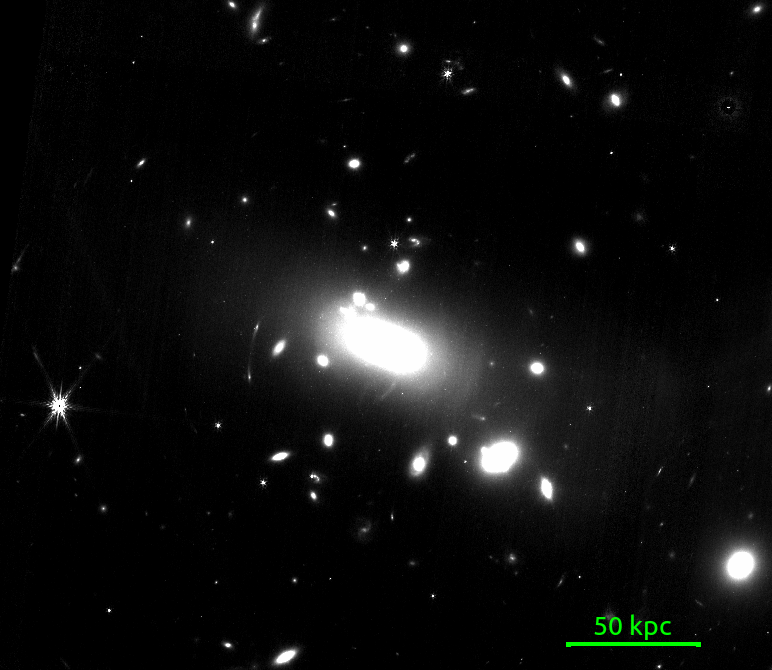
\includegraphics[trim={0 0 0 0}, clip, width=0.45\textwidth]{bcg200b.png}
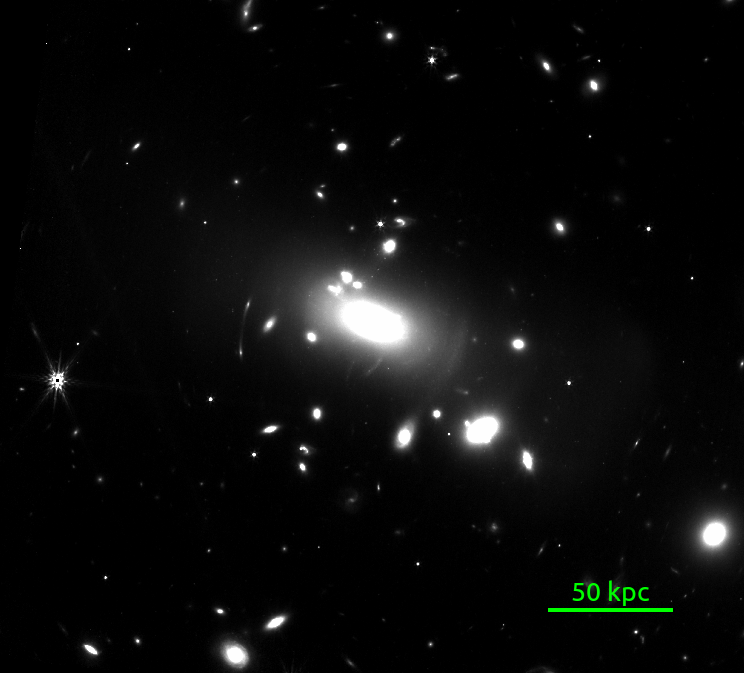
\includegraphics[trim={0 0 0 20}, clip, width=0.45\textwidth]{bcg277b.png}		
%
\includegraphics[trim={100 100 100 100}, clip, width=0.45\textwidth]{escudoUGRnew.jpg}	
\caption{Imágenes del entorno de la BCG de \clust{} con los filtros F200W (izquierda) y F277W (derecha), ambos con una escala de 0 a 1 MJy/sr. Alrededor de la BCG existe un halo tenue con forma alargada, dentro del cual se aprecian algunas estructuras que podrían ser shells. \label{bcg}}
\end{figure}
\noindent


\begin{figure}[h]
\centering
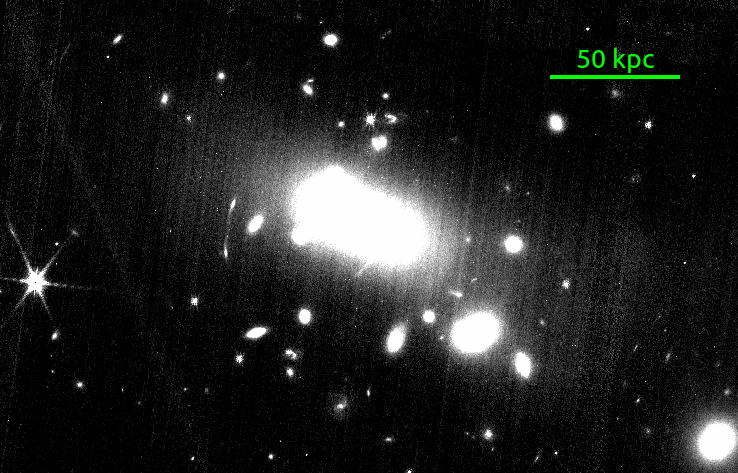
\includegraphics[trim={0 0 0 0}, clip, width=0.6\textwidth]{bcg115b.png}	
%
\includegraphics[trim={0 0 0 300}, clip, width=0.6\textwidth]{escudoUGRnew.jpg}	
\caption{Imagen de la BCG en el filtro F115W con una escala de 0 a \(0,3\) MJy/sr, en la que se observan de manera muy clara los artefactos que contaminan las imágenes del canal SW de JWST. También se distingue la forma rectangular de la ICL en el lado oeste, en contraste con el más redondeado extremo este. \label{bcg115}}
\end{figure}
\noindent


\begin{figure}[h]
\centering
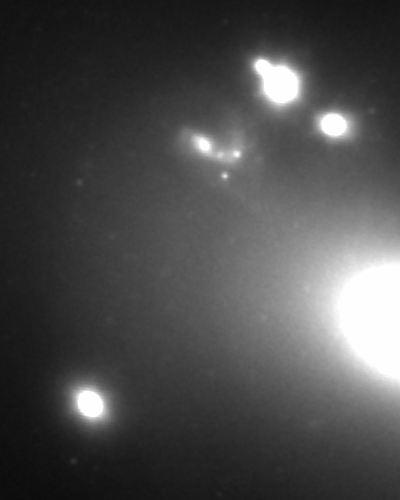
\includegraphics[trim={0 0 0 0}, clip, width=0.4\textwidth]{galaxias.png}
\caption{Imagen del filtro F277W de las galaxias presentes en el costado este de la BCG a una escala de 0-2 MJy/sr. Se distinguen claramente una galaxia al sur y tres al norte. Cerca del centro vemos cuatro puntos luminosos diferenciados que pueden tratarse un pequeño grupo de galaxias. El que está situado más al oeste forma una cola visible que se extiende al norte del grupo. Si cada uno de esos puntos brillantes representa una galaxia individual, observamos un total de ocho. \label{fig:galaxias}}
\end{figure}
\noindent




\subsection{Datos de HST}
El Telescopio Espacial Hubble también observó \clust{} a través del programa CLASH \citep{postmanClusterLensingSupernova2012} con las cámaras ACS y WFC3. Con la primera se utilizaron ocho filtros del rango óptico e infrarrojo cercano con el canal WFC, mientras que con la segunda se obtuvieron datos en cinco bandas infrarrojas con el canal IR y cuatro ultravioletas con el canal UVIS. Sin embargo, como indicaron \citet{jimenez-tejaFirstJointMUSE2024}, en el canal UVIS no se aprecian las características de bajo brillo superficial como la ICL, y las imágenes del filtro F555W de ACS no cubren la zona de la BCG. Por lo tanto, en total contamos con las cinco imágenes del canal IR de WFC3 y siete de ACS. En la Tabla \ref{tab:hst} podemos ver un resumen de las características de los filtros utilizados y las medidas asociadas\footnote{\url{https://hst-docs.stsci.edu/acsihb/chapter-5-imaging/5-1-imaging-overview}}\(^{,}\)\footnote{\url{https://hst-docs.stsci.edu/hpiom/chapter-12-wide-field-camera-3-wfc3/12-5-wfc3-reference-information/12-5-2-wfc3-ir-spectral-elements}}. Según se indica en el \textit{header} de los archivos, la ganancia de la cámara ACS es de 2,0 \(e^- /\)ADU, y la de WFC3/IR de 2,0 \(e^- /\)ADU. Por su parte, la escala de píxeles de todas las medidas es de 0,03 arcsec/píxel. \par

\begin{table}[]
\centerline{
\begin{tabular}{|c|c|c|c|c|}
\hline
Telescopio/Cámara/Canal      & Filtro &  \begin{tabular}{c} $\lambda$ \\ (nm) \end{tabular}  & \begin{tabular}{c} $\Delta \lambda$ \\ (nm) \end{tabular} & \begin{tabular}{c} Exposición \\ (s) \end{tabular}  \\ \hline
\multirow{7}{*}{HST/ACS/WFC} & F435W  & 429,7          & 103,8                 & 3910  \\ \cline{2-5}
                             & F475W  & 476,0          & 145,8                 & 3728  \\ \cline{2-5}
                             & F606W  & 590,7          & 234,2                 & 3870  \\ \cline{2-5}
                             & F625W  & 631,8          & 144,2                 & 3728  \\ \cline{2-5}
                             & F775W  & 776,4          & 152,8                 & 7792   \\ \cline{2-5}
                             & F814W  & 833,3          & 251,1                 & 7866   \\ \cline{2-5}
                             & F850LP & 944,5          & 122,9                 & 15084   \\ \cline{1-5} 
\multirow{5}{*}{HST/WFC3/IR} & F105W  & 1048,95        & 292,30                & 2614   \\ \cline{2-5}
                             & F110W  & 1141,40        & 503,40                & 2414  \\ \cline{2-5}
                             & F125W  & 1245,90        & 301,50                & 3420     \\ \cline{2-5}
                             & F140W  & 1392,10        & 399,00                & 2311     \\ \cline{2-5}
                             & F160W  & 1540,52        & 287,88                & 6238    \\ \hline
\end{tabular}}
\caption{Algunas características relevantes de las medidas tomadas con HST. \label{tab:hst}}
\end{table}

Los datos descargados\footnote{\url{https://archive.stsci.edu/prepds/clash/}} ya se procesaron mediante la \textit{pipeline} de la colaboración CLASH, que es adecuada para el estudio de objetos de bajo brillo superficial \citep{jimenez-tejaRELICSICLAnalysis2021,jimenez-tejaFirstJointMUSE2024}. La medida empírica en cada píxel se expresa en unidades de electrones por segundo (e\(^{-}\)/s). \par

Las imágenes de WFC3/IR cubren aproximadamente el mismo rango de longitudes de onda que el canal SW de JWST, por lo que las imágenes son muy similares. En los filtros ópticos de ACS, sin embargo, tenemos varios cambios. En la Figura \ref{bcgacs} representamos la BCG vista con el filtro F606W (izquierda) y F435W (derecha), con una escala de 0 a \(0,05 \: \text{e}^{-}/\text{s}\). Es evidente que hay un descenso abrupto de la luminosidad al acercarnos al azul provocado por el alto redshift del cúmulo, de modo que las shells se vuelven indistinguibles. Las imágenes de ACS, por lo tanto, no son adecuadas para identificar las shells. También se vuelven más tenues las galaxias que identificábamos antes. La que está situada más al noroeste (a la derecha), de hecho, no se distingue en ninguno de los dos filtros, lo que sugiere que tiene un espectro más rojo que las demás. En efecto, en el catálogo de objetos de CLASH esta galaxia (ID 760) se sitúa a un redshift \(0,937 \leq z \leq 1,029\), mucho mayor que el del resto. 

\begin{figure}[h]
\centering
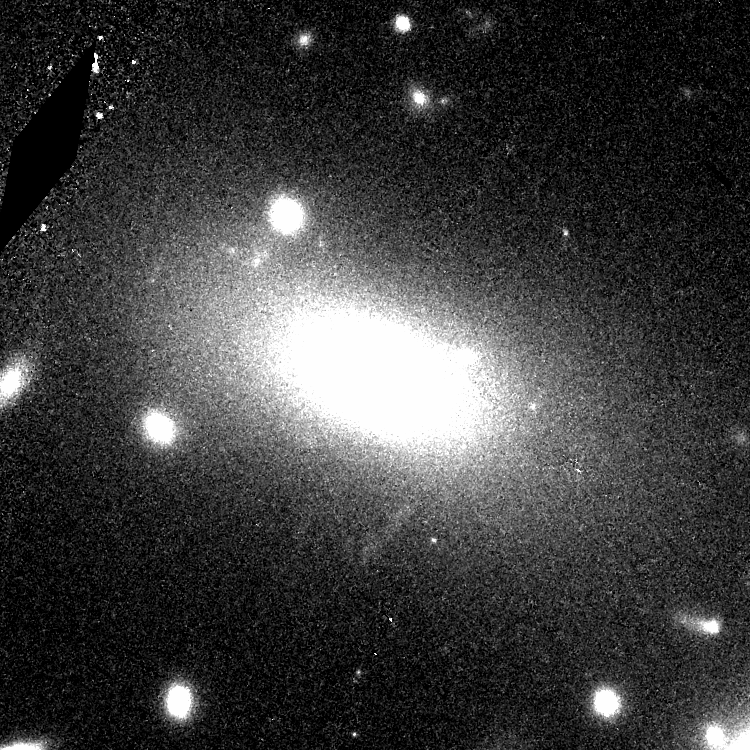
\includegraphics[trim={0 0 0 0}, clip, width=0.45\textwidth]{bcg606.png}
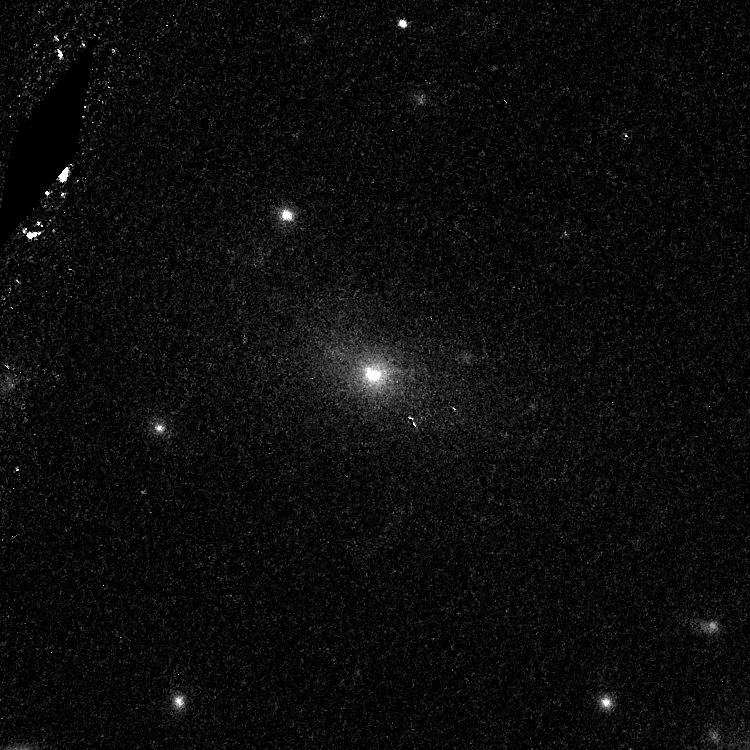
\includegraphics[trim={0 0 0 0}, clip, width=0.45\textwidth]{bcg435.png}		
\caption{Imágenes de los filtros F606W (izquierda) y F435W (derecha) de HST/ACS, ambas con una escala de 0 a \(0,05 \: \text{e}^{-}/\text{s}\). En estas longitudes de onda las emisiones son mucho más tenues, y ya no es posible hablar de shells. Además, una de las galaxias que contaminaba la luz de la BCG desaparece por completo debido a que se encuentra a una distancia mucho mayor y, por lo tanto, tiene un espectro desplazado al infrarrojo. \label{bcgacs}}
\end{figure}
\noindent


\subsection{Datos de VLT MUSE}
MUSE es un espectrógrafo de alta resolución\footnote{\url{https://www.eso.org/sci/facilities/paranal/instruments/muse/overview.html}} instalado en el VLT del Observatorio Paranal en Chile\footnote{\url{https://www.eso.org/public/spain/teles-instr/paranal-observatory/vlt/}}, perteneciente al ESO. A través de 24 Integral Field Units (IFU) permite caracterizar el espectro de una región del espacio entre longitudes de onda de 475 y 935 nm, por lo que es una herramienta excelente para analizar las emisiones ópticas de los objetos astrofísicos. En el llamado Wide Field Mode, cada medida genera 3681 imágenes con una distancia entre longitudes de onda características de 1,25 nm, lo que se traduce en un poder de resolución de entre 1770 y 3590. En este modo, el instrumento cuenta con un campo de visión de 1 arcmin\(^{2}\) y una escala de píxeles de 0,2 arcsec/píxel. \par

MUSE identificó \clust{} como un cúmulo de gran interés para las medidas de espectroscopía, y por ello varios programas lo han observado durante un tiempo total acumulado de 20720 s. Esta exposición es suficiente para formar parte de la colección MUSE-DEEP\footnote{\url{https://doi.org/10.18727/archive/42}}, que engloba las medidas más profundas de MUSE. En la Figura \ref{musejimteja} podemos ver una composición de las observaciones en todas las longitudes de onda. \par


\begin{figure}[h]
\centering
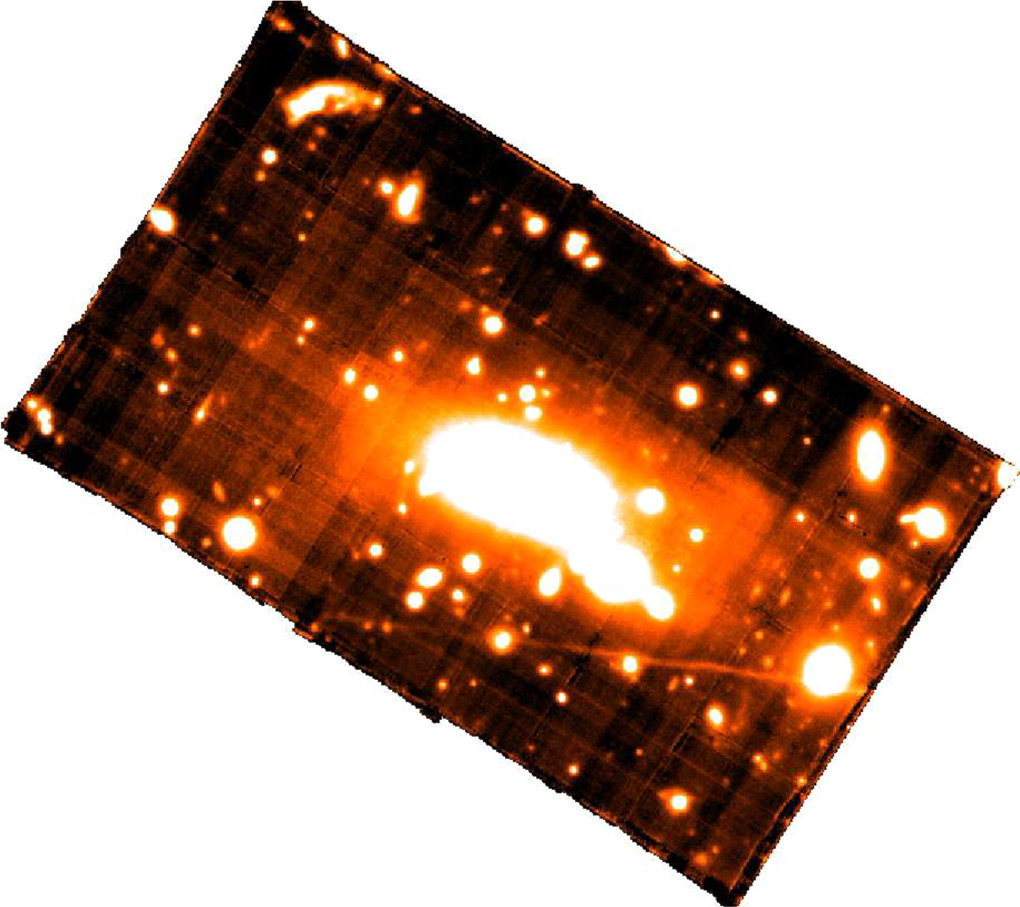
\includegraphics[trim={0 0 0 0}, clip, width=0.5\textwidth]{musejimteja.jpg}	
\caption{Composición sobre todas las longitudes de onda de las imágenes de \clust{} tomadas por MUSE. Imagen de \citet[fig. 3]{jimenez-tejaFirstJointMUSE2024}.\label{musejimteja}}
\end{figure}
\noindent

Las imágenes de MUSE descargadas ya fueron procesadas por el equipo del ESO y se presentan en unidades de \(10^{-20}\: \text{erg}\: \text{s}^{-1}\: \text{cm}^{-2}\: \text{\AA}^{-1}\), de modo que, de la misma manera que con los datos de JWST y HST, no fue necesario tener en cuenta la calibración del detector. Sin embargo, sí existe una diferencia fundamental entre los datos de MUSE y los procedentes de los telescopios espaciales: la señal telúrica (terrestre). La atmósfera absorbe y emite la luz en determinadas longitudes de onda y contamina los espectros medidos, especialmente aquellos producidos por objetos de bajo brillo superficial. Para solucionar este problema utilizamos el software ZAP \citep[Zurich Atmosphere Purge,][]{sotoZAPEnhancedPCA2016}, que analiza el espectro completo y suprime, en la medida de lo posible, las líneas espectrales atmosféricas. \label{sec:muse}